\chapter{Evaluation}

In previous chapters, we have made fairly extensive reasoning behind each part of the algorithm. However, we have yet to see how the algorithm will perform as a whole. In this chapter, the algorithm is tested in various situations.

Since the quality of the approach cannot simply be measured with respect to the number of joints or obstacles, we evaluate various aspects in different environments. First, we handcraft various situations for the manipulator, and show the performed movement. Then, we take a look at the different components of the algorithm and analyze how much time is spent in each of them, in order to look for possible improvements. Finally, we explore the limits in the respective types of environments.

\section{Case Study}\label{study}

First part of the evaluation consists of putting the algorithm up against handcrafted sets of obstacles. We can view how particular edge cases are handled, how natural the overall motion is, and if there are any situations it cannot reasonably deal with.

We can now demostrate initial results within a RoFI simulator. As a baseline, we consider a manipulator that consists of a chain of 4 modules, linked via the $-Z$ connectors. Since such a manipulator has 12 degrees of freedom, previous state of the art algorithms -- which mostly only scale up to 6 DoF -- would clearly not be useful.
The simulator does not consider the forces of gravity, or physical failure of the modules; these are aspects of further research. The reasoning behind using 4 modules as the baseline is that such a manipulator is flexible enough even though the joints are constrained, and with the state of the art hardware, it's feasible for the joint of a single module to lift the weight of around 3 connected modules, but not significantly more.

The measurements take place on consumer grade hardware, equipped with 16 GB RAM and an Intel Core i7-8750H cpu.

To evaluate the quality of the algorithm, we want to explore how differently shaped environments affect the algorithm's runtime and ability to find successful paths.

As a sanity check, we can start with a simple case of a target near an obstacle, but reachable from the initial position. The environment is a wall made out of 12 small spheres. Figure~\ref{fig:sim3} shows the performed movement.

\begin{figure}
  \centering
  \begin{minipage}{\textwidth}
    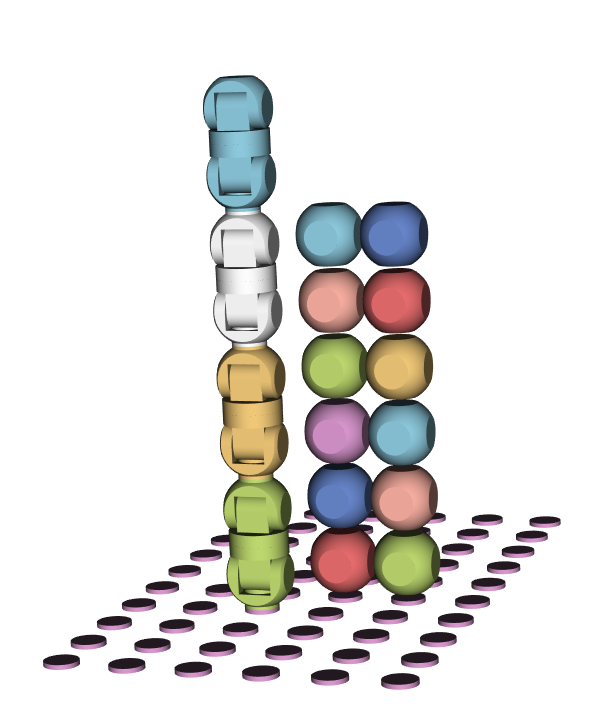
\includegraphics[width=0.24\textwidth]{sim3_0.png}
    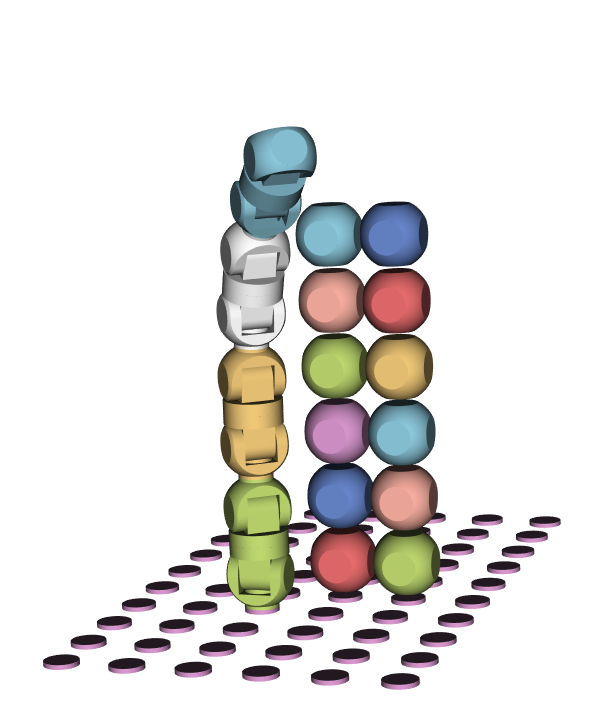
\includegraphics[width=0.24\textwidth]{sim3_1.png}
    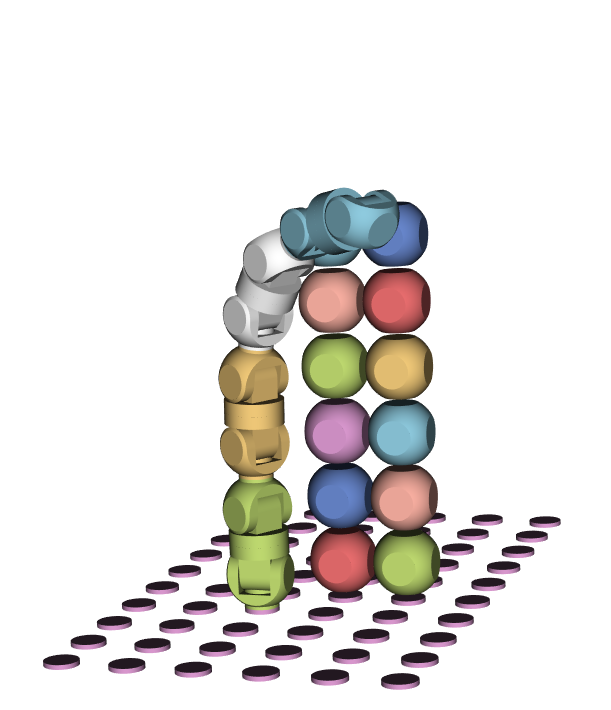
\includegraphics[width=0.24\textwidth]{sim3_2.png}
    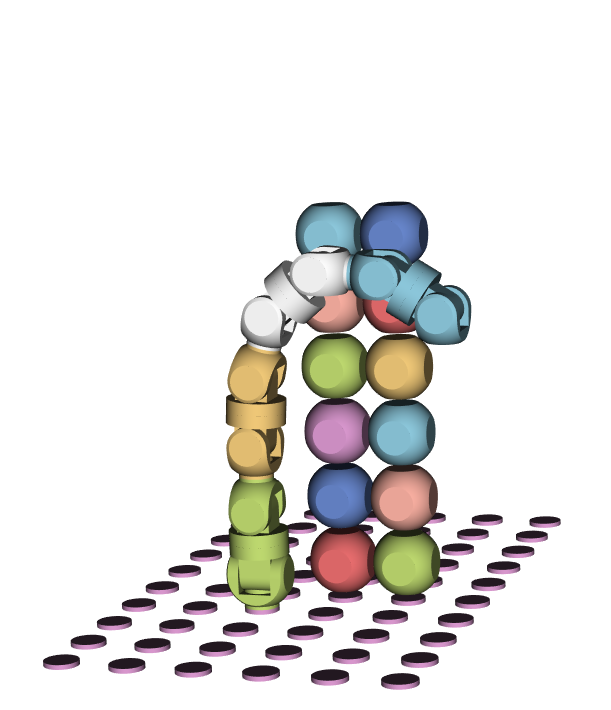
\includegraphics[width=0.24\textwidth]{sim3_3.png}
  \end{minipage}
  \caption{Target near obstacle}\label{fig:sim3}
\end{figure}

A notable feature observable in this case is that even though there is a fairly high number of obstacles, they do not affect the final result in a negative way unless they are in the way. The final position looks very natural, and the performed movement is as smooth as it gets: a direct interpolation between the initial and target position. Since the target is visible from the initial position, the algorithm directly finds the path from it to the target. The whole computation runs for around $0.01$ second.

\begin{figure}[ht]
  \centering
  \begin{minipage}{0.9\textwidth}
    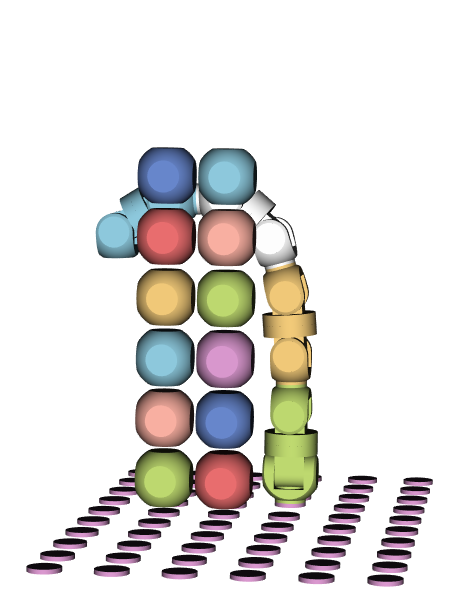
\includegraphics[width=0.24\textwidth]{sim4_0.png}
    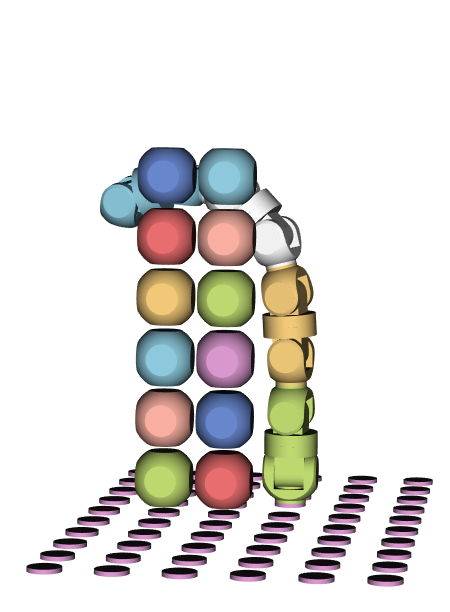
\includegraphics[width=0.24\textwidth]{sim4_1.png}
    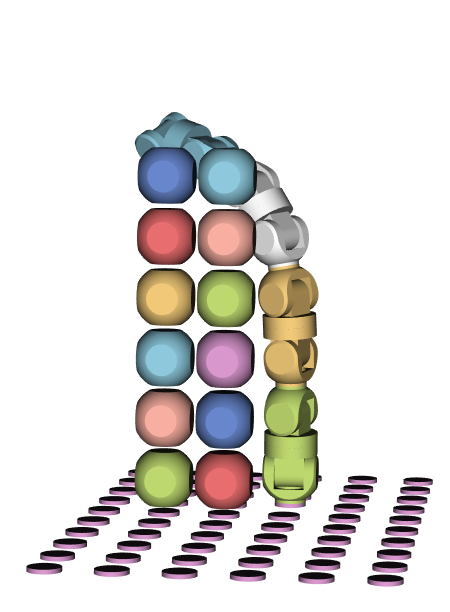
\includegraphics[width=0.24\textwidth]{sim4_2.png}
    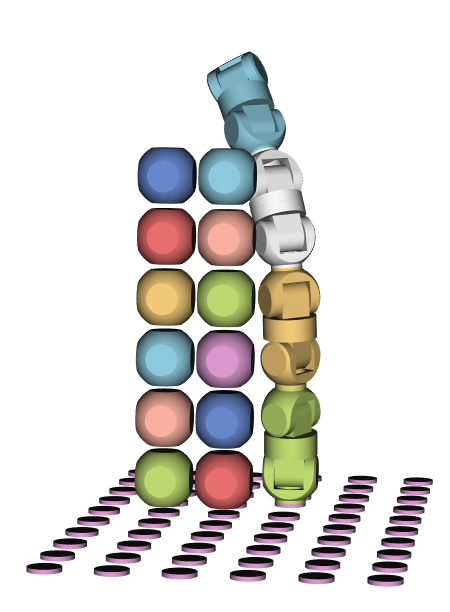
\includegraphics[width=0.24\textwidth]{sim4_3.png}

    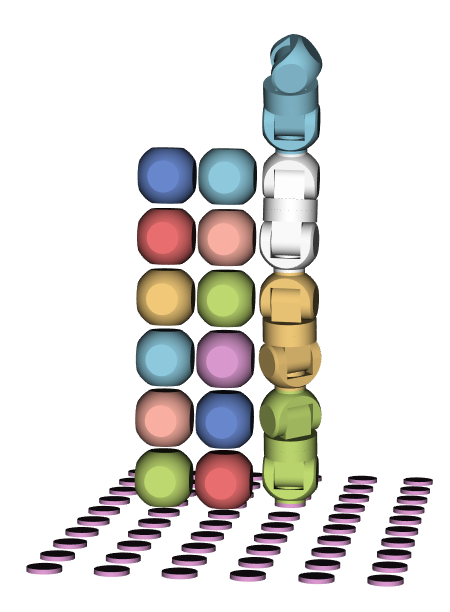
\includegraphics[width=0.24\textwidth]{sim4_4.png}
    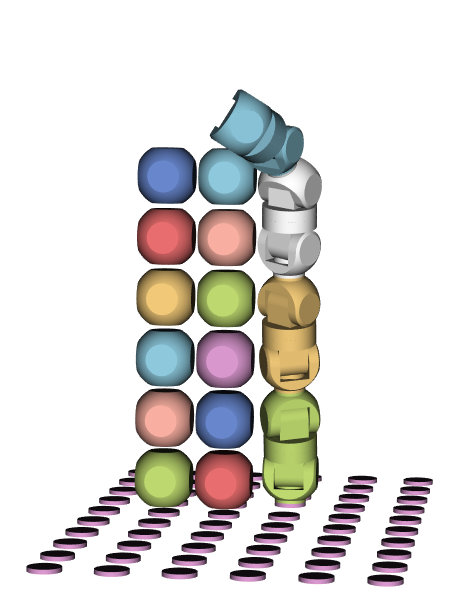
\includegraphics[width=0.24\textwidth]{sim4_5.png}
    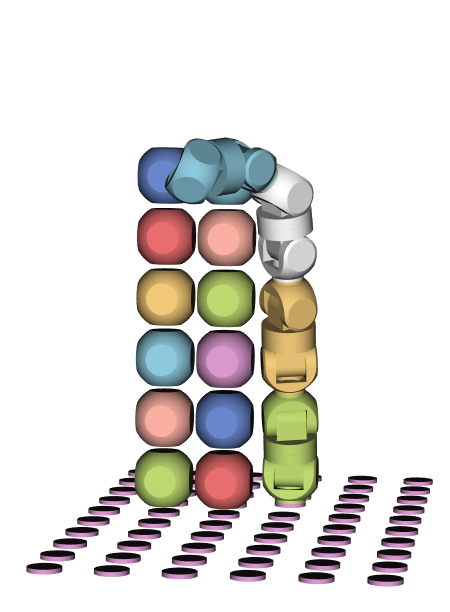
\includegraphics[width=0.24\textwidth]{sim4_6.png}
    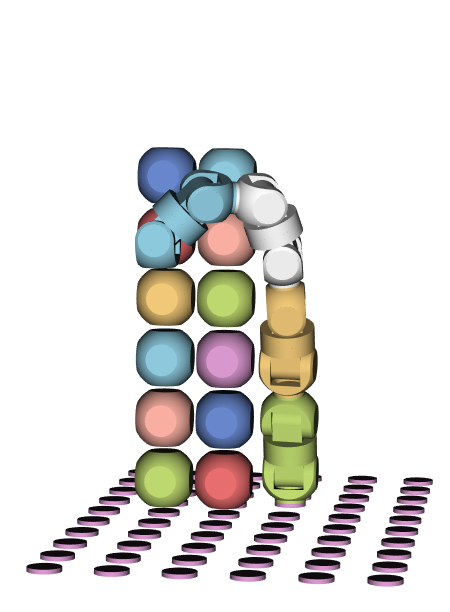
\includegraphics[width=0.24\textwidth]{sim4_7.png}
  \end{minipage}
  \caption{Target behind obstacle}\label{fig:sim4}
\end{figure}

A more interesting case is observable when we start off in a position close to the wall and try to reach a target behind the wall. In this case, the algorithm needs to first move back to avoid the wall, and then go to the target. The direct path can no longer be taken due to the obstacles, and going around the wall is infeasible due to the limited length of the manipulator. A possible motion generated by the algorithm can be seen in Figure~\ref{fig:sim4}.

Unlike the first test case, the algorithm does not immediately find the right path. Since the paths that lead behind the wall are physically closer, they are evaluated as shorter at first, but trying to folow them fails due to the limited length of the manipulator. On the 3\rd{} path, a correct solution that goes around the wall is found. Since we needed to explore multiple paths, each of which is associated with a lot of computation, the solution was found in $0.5$ seconds.

The next test case consists of trying to fit the manipulator in a small hole between obstacles and reach a target behind it. In some cases, this problem has proven to be challenging.
Any path to the target has to go through the hole, but the direction where we come from can play a part as well: in order to fit the joints through the hole, the manipulator needs to move in a fairly specific direction, because there is not enough space to move around and readjust when the manipulator goes through the hole. Usually, it does find a solution, see Figure~\ref{fig:sim5}.


\begin{figure}[ht]
  \centering
  \begin{minipage}{\textwidth}
    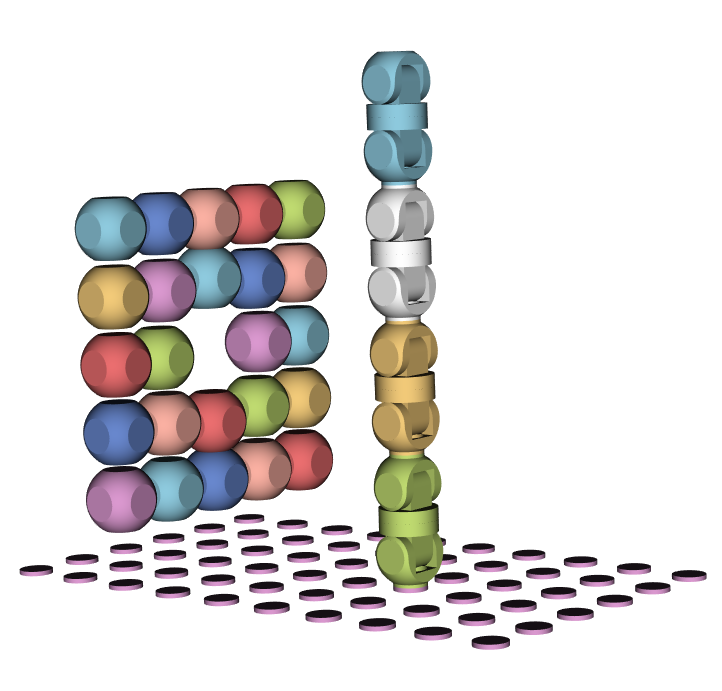
\includegraphics[width=0.24\textwidth]{sim5_0.png}
    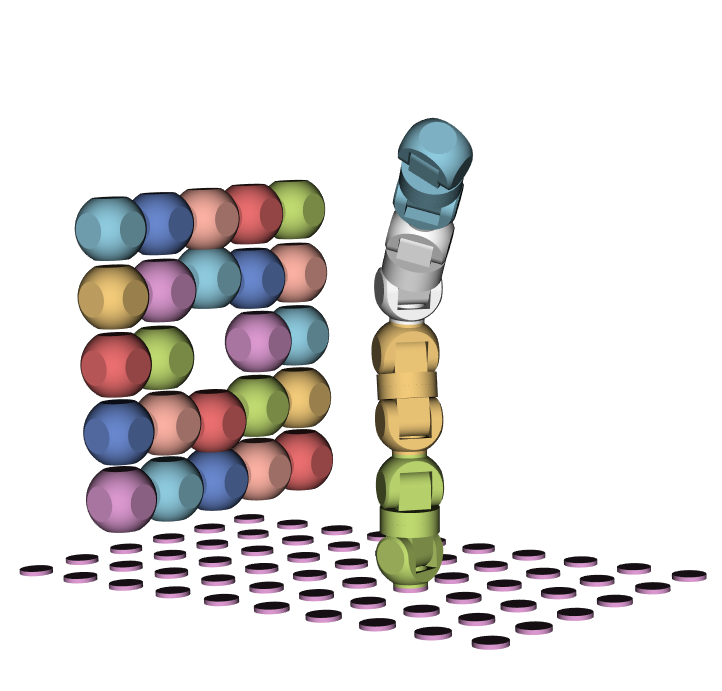
\includegraphics[width=0.24\textwidth]{sim5_1.png}
    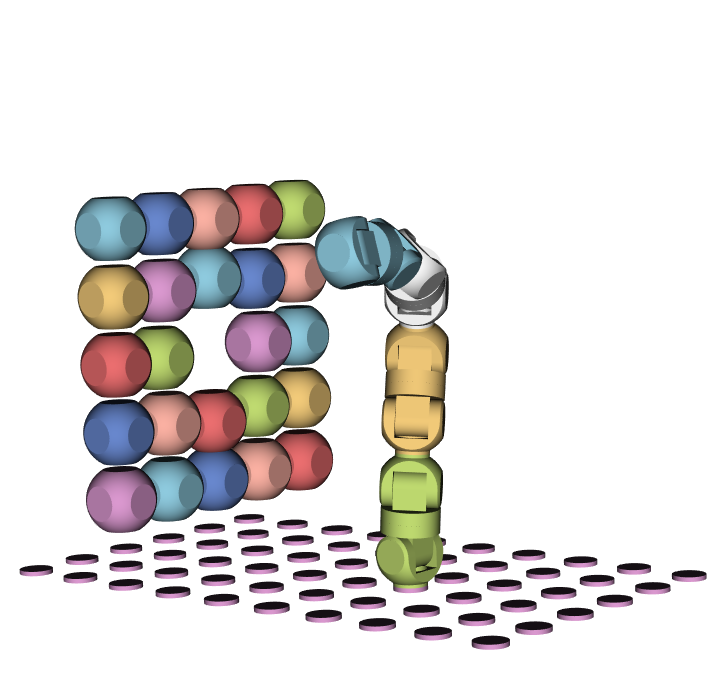
\includegraphics[width=0.24\textwidth]{sim5_2.png}
    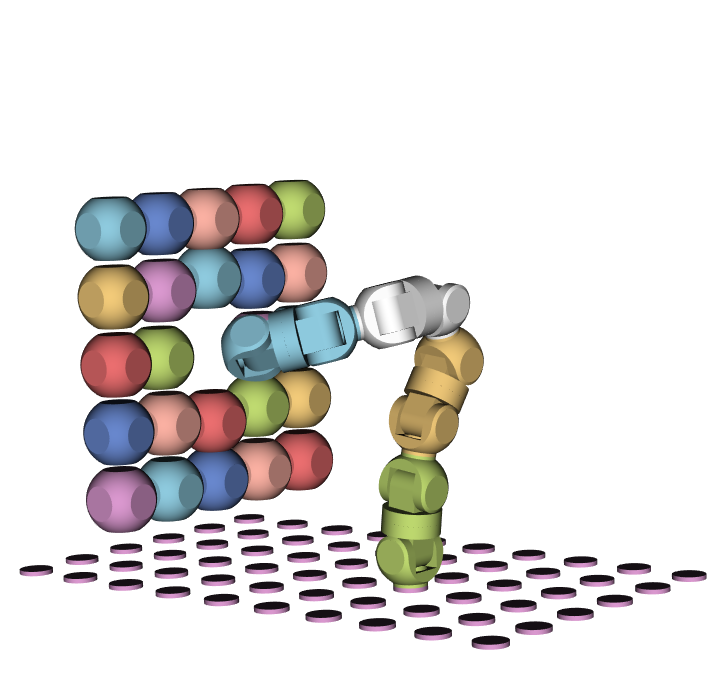
\includegraphics[width=0.24\textwidth]{sim5_3.png}

    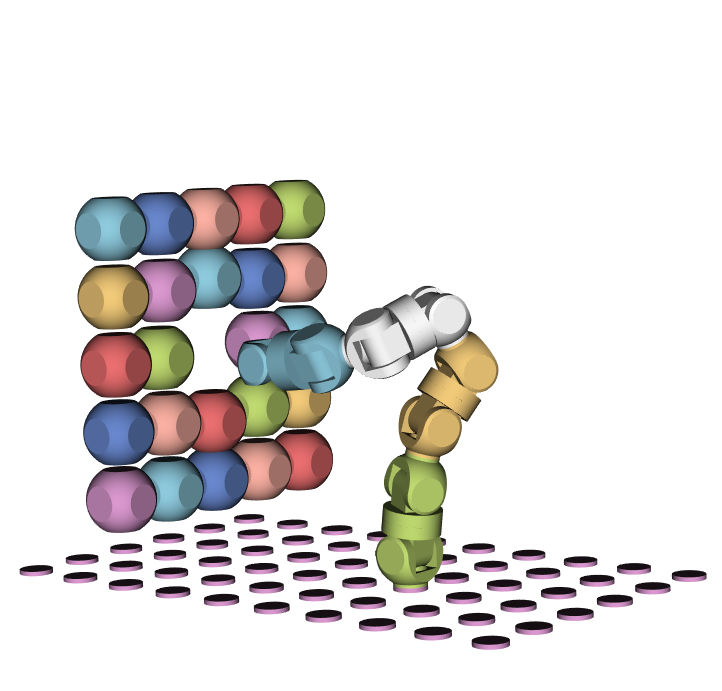
\includegraphics[width=0.24\textwidth]{sim5_4.png}
    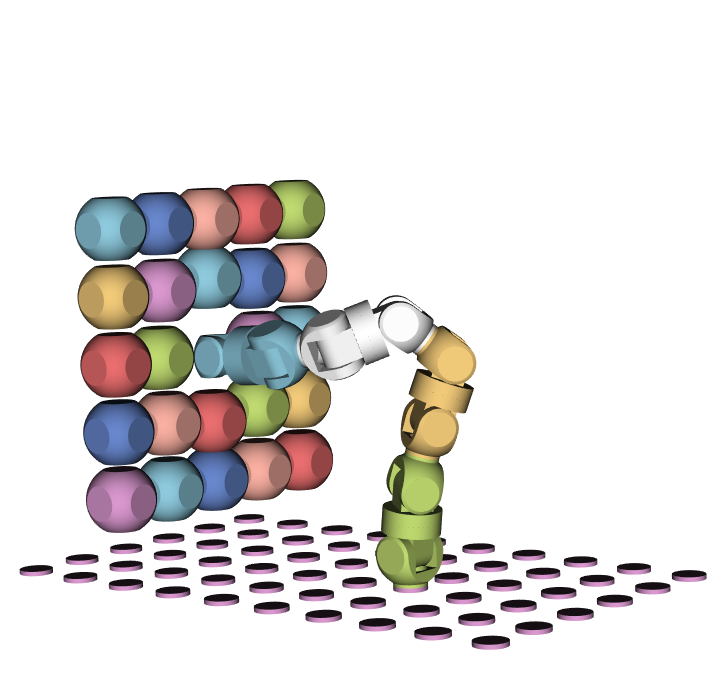
\includegraphics[width=0.24\textwidth]{sim5_5.png}
    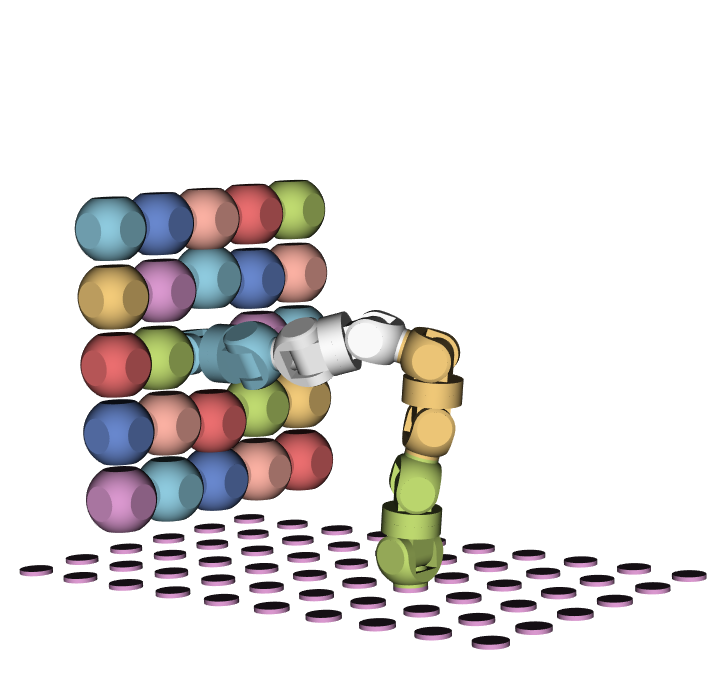
\includegraphics[width=0.24\textwidth]{sim5_6.png}
    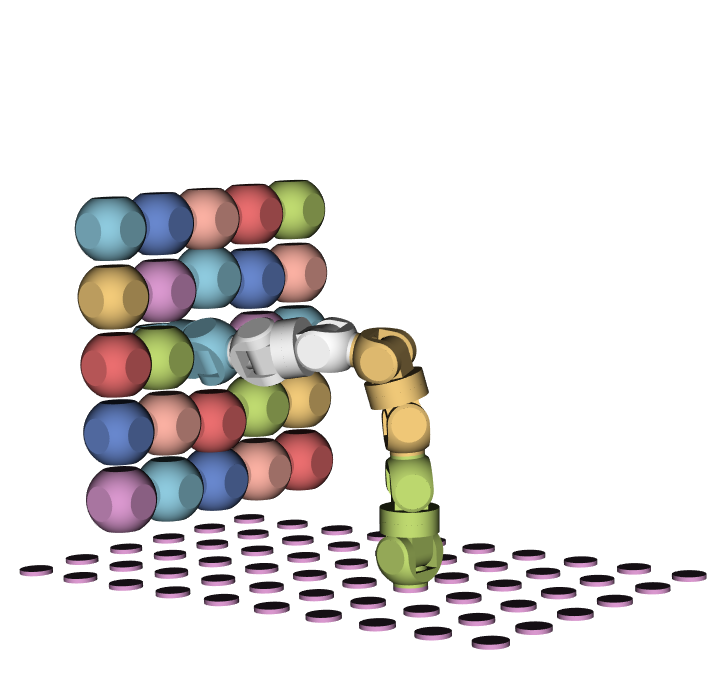
\includegraphics[width=0.24\textwidth]{sim5_7.png}
  \end{minipage}
  \caption{Hole between obstacles}\label{fig:sim5}
\end{figure}

However, if the target is fairly far beyond the hole, but the only way to reach it is to go through it, the algorithm does struggle. Since the point between the obstacles is associated with a high cost, it often tries other paths first, exploring a much larger part of the space compared to the previous examples.

The example~\ref{fig:sim5} was found in $0.04$ seconds, on the first explored path. However, some targets further from the hole can lead to exploring a much larger number of paths; leading to a noticeable delay of a few seconds.

% As it stands, the algorithm has its limits. One particular case where it fails to find a viable path in a reasonable time\footnote{The algorithm shuts down after 100 explored paths, which corresponds to up to half a minute of computation time, depending on the complexity of the environment.} is when there is a big wall right in front of the initial \textit{end effector} position, and another one behind it. In our example, see Figure~\ref{fig:d_wall}, we have a floating wall, followed by a small wall, and the target lies beyond both. To reach the goal, the manipulator would have to perform a very complex and specific motion: reach back, curl up under the first wall, go between the walls, and finally reach the goal. Unfortunately, due to how the algorithm works and how constants are set, the manipulator keeps trying to find ways around the walls, with no success. Paths that go down the wall fail due to the fact that there isn't enough space between the manipulator and the wall, and it cannot assume the positions in a natural way.

% \begin{figure}
%   \centering
%   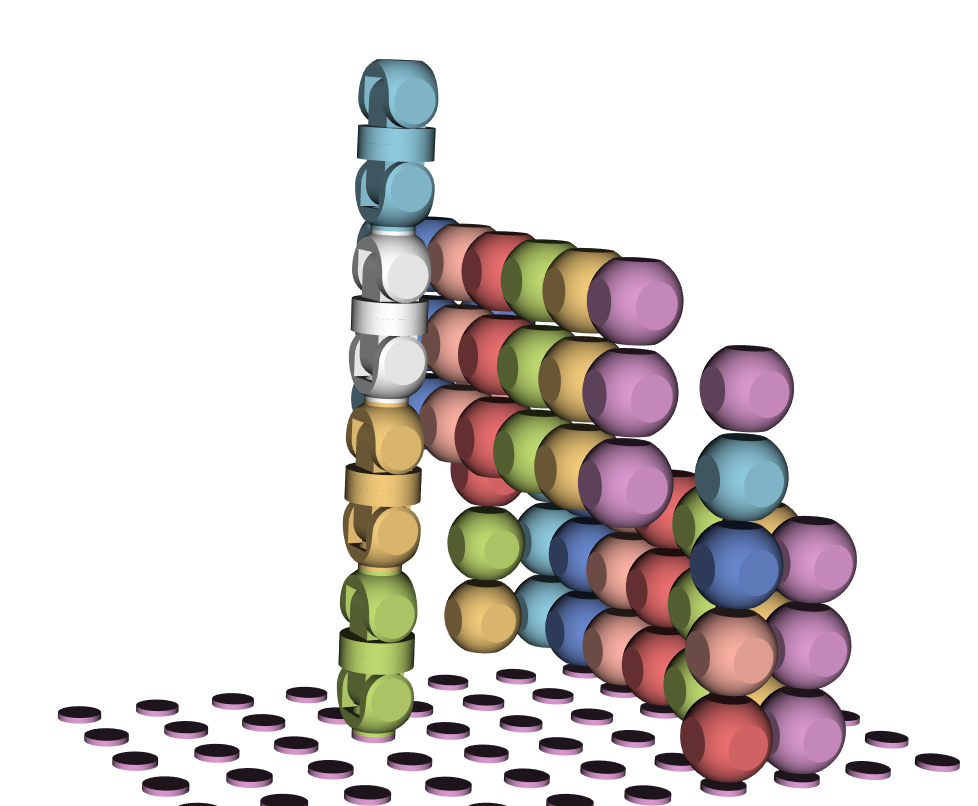
\includegraphics[width=0.5\textwidth]{double_wall.png}
%   \caption{Test case 4: Double wall with complex motion}\label{fig:d_wall}
% \end{figure}

% With minor modifications to the problem, the algorithm does find a viable solution, which gives us some hints for future improvements. The cases where it does find solutions to the problem are:

% \begin{itemize}
% \item The first wall is a bit further from the manipulator.
% \item The walls are not as wide and there is a way around them.
% \item The manipulator is not in a straightened out position, but already somewhat curled up at the start of the computation.
% \end{itemize}

Moving on, we want to see how the algorithm performs when the obstacles do not form a wall, but instead float in space and form clusters. First up, clusters near the target. This is clearly a practically motivated problem: if we have some objects lying around and need to pick and place a specific one (or a few), we require a precise motion that avoids the other objects.

\begin{figure}[ht]
  \centering
  \begin{minipage}{0.85\textwidth}
    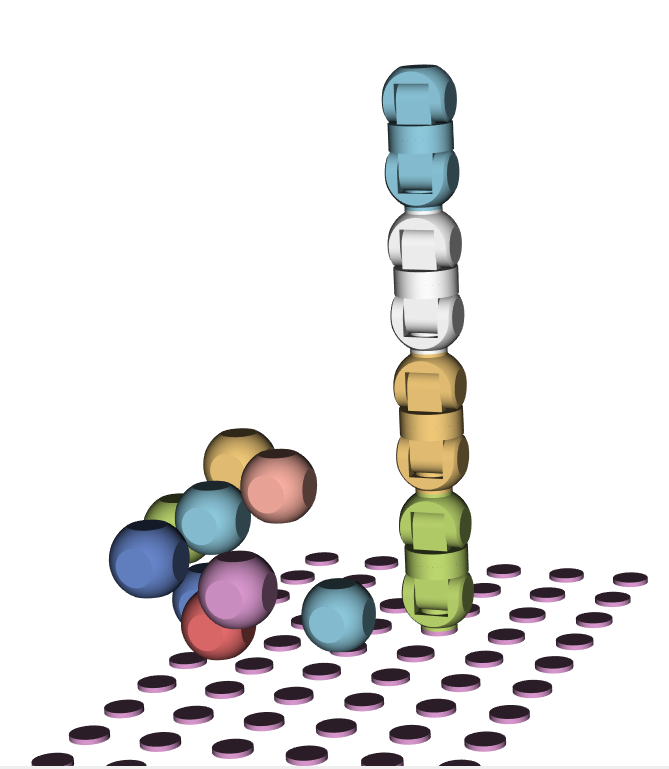
\includegraphics[width=0.33\textwidth]{sim6_0.png}
    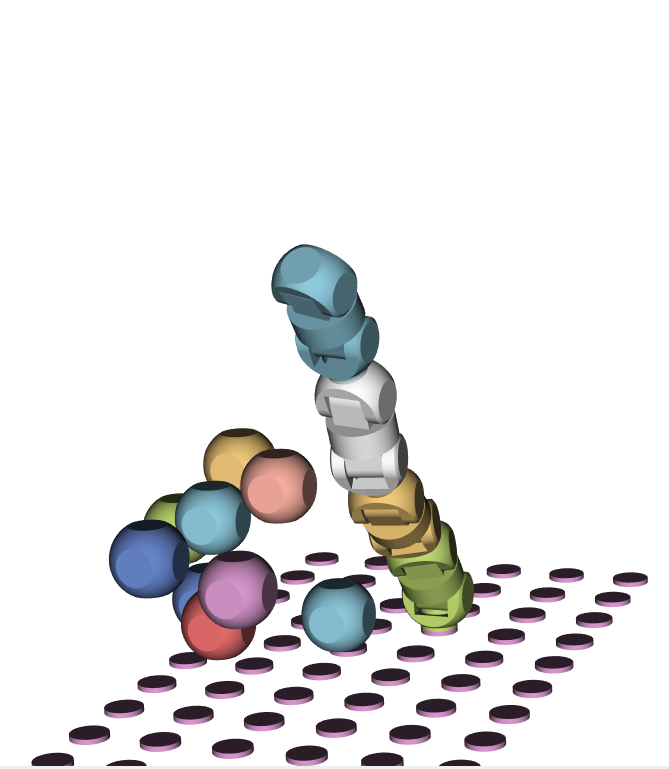
\includegraphics[width=0.33\textwidth]{sim6_1.png}
    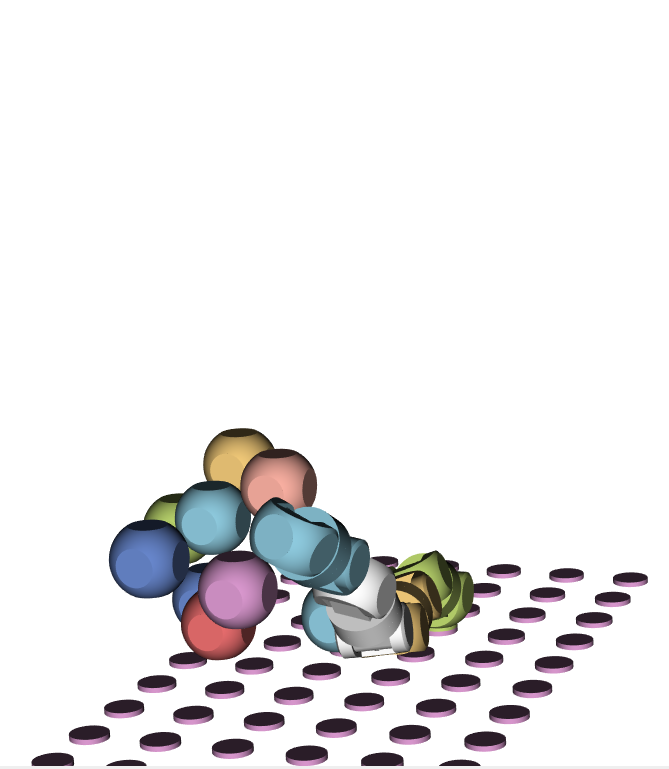
\includegraphics[width=0.33\textwidth]{sim6_2.png}

    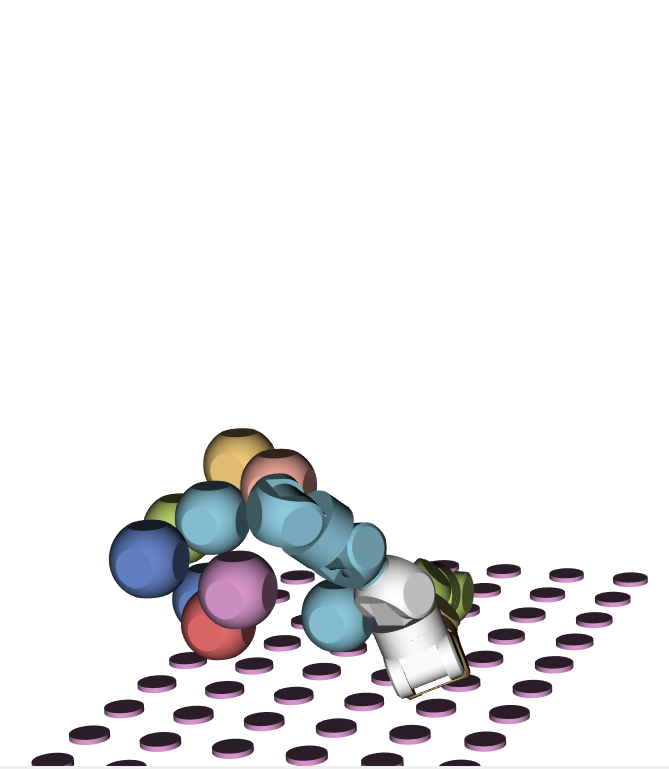
\includegraphics[width=0.33\textwidth]{sim6_3.png}
    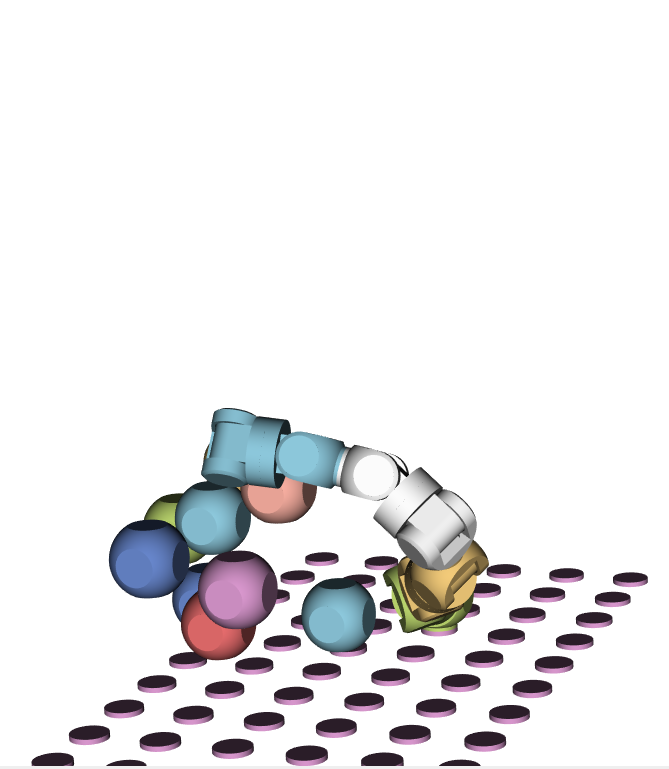
\includegraphics[width=0.33\textwidth]{sim6_4.png}
    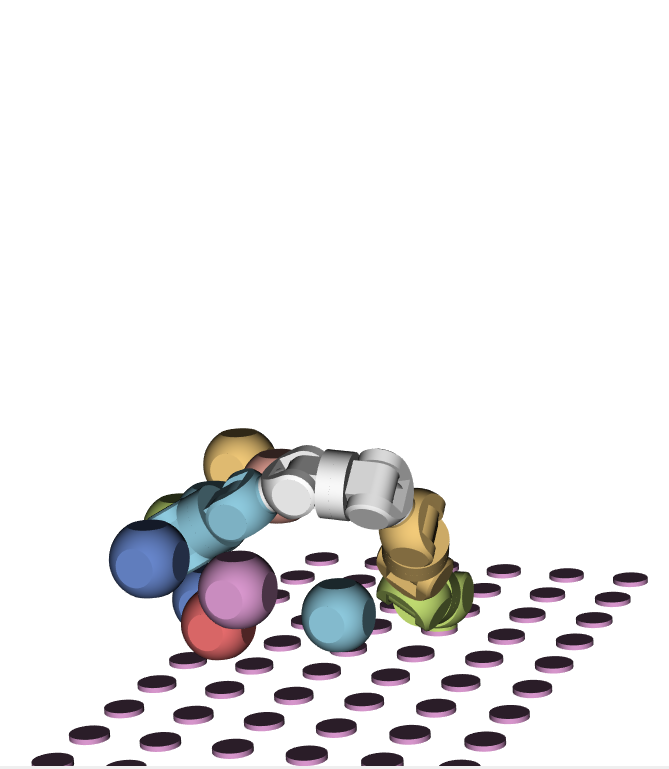
\includegraphics[width=0.33\textwidth]{sim6_5.png}
  \end{minipage}
  \caption{Getting around clusters of objects}\label{fig:sim6}
\end{figure}

The algorithm acts as expected, finding quick and natural looking solutions. Figure~\ref{fig:sim6} shows one example of getting around and between obstacles to reach a target. As designed, the algorithm prioritizes paths that avoid the obstacles altogether and only goes between them at the end of the path if necessary. This often leads to the first evaluated path being correct, which leads to a result in around $0.02$ seconds. When the target lies right in the middle of a cluster and is difficult to navigate into, the algorithm explores multiple paths, but still finishes in less than a second.

Finally, we can take a look at how obstacles affect the manipulator when they are not close to the manipulator's \textit{end effector}, but rather the lower joints of the manipulator. When the obstacles are all around the manipulator, they do not have as great of an effect on the found paths, compared to when they are surrounding the target. As a result, we need to rely on the quality of our extended FABRIK to avoid them.

\begin{figure}
  \centering
  \begin{minipage}{\textwidth}
    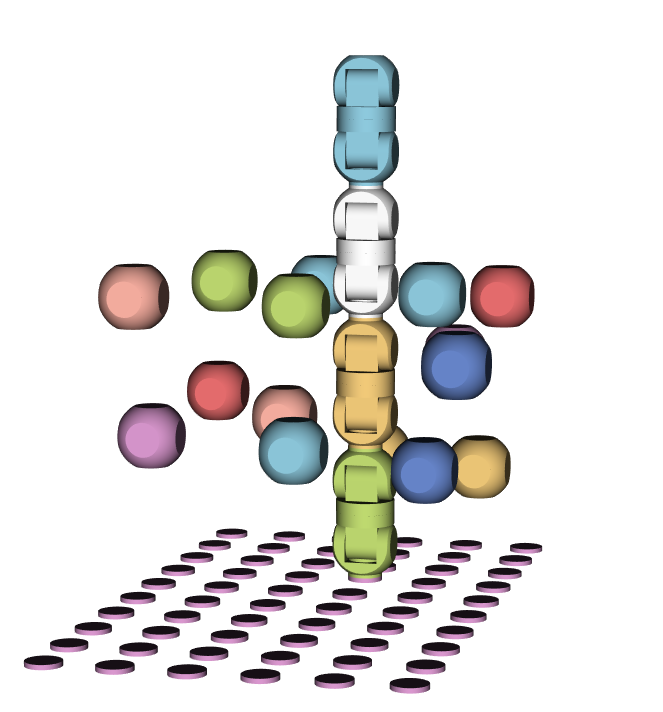
\includegraphics[width=0.245\textwidth]{sim7_0.png}
    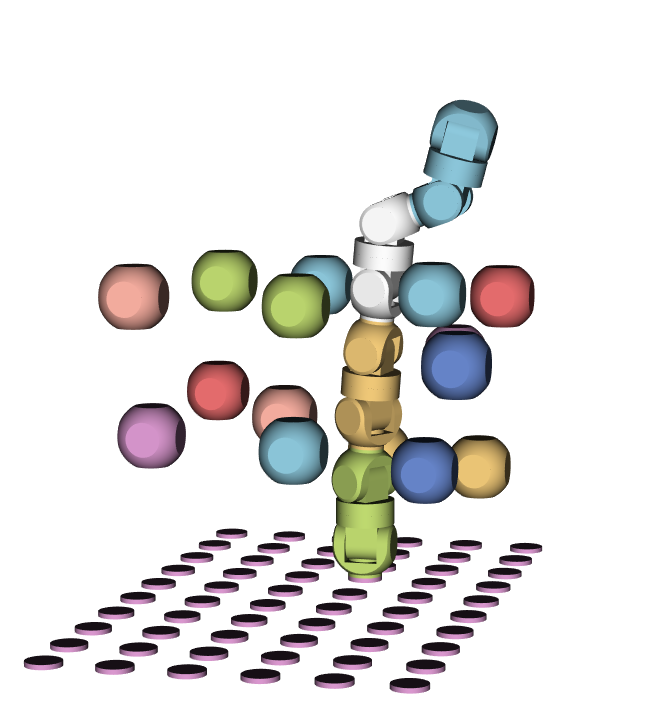
\includegraphics[width=0.245\textwidth]{sim7_1.png}
    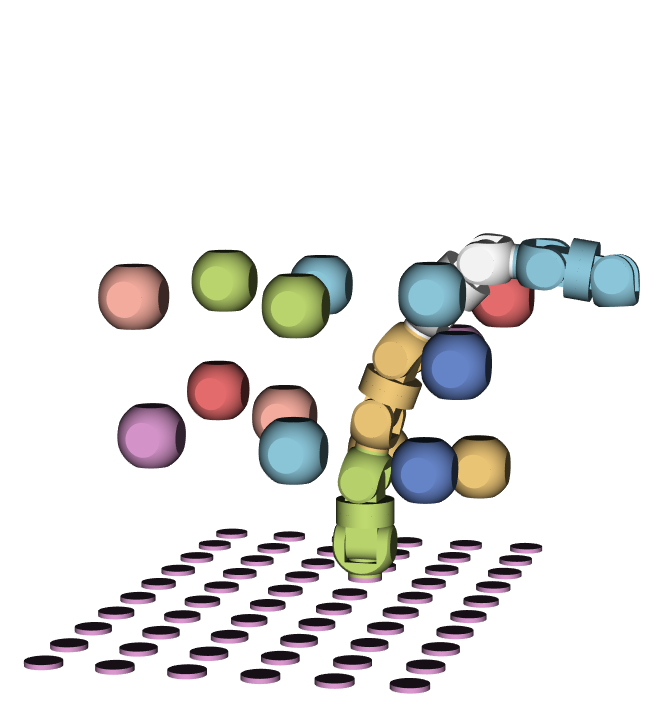
\includegraphics[width=0.245\textwidth]{sim7_2.png}
    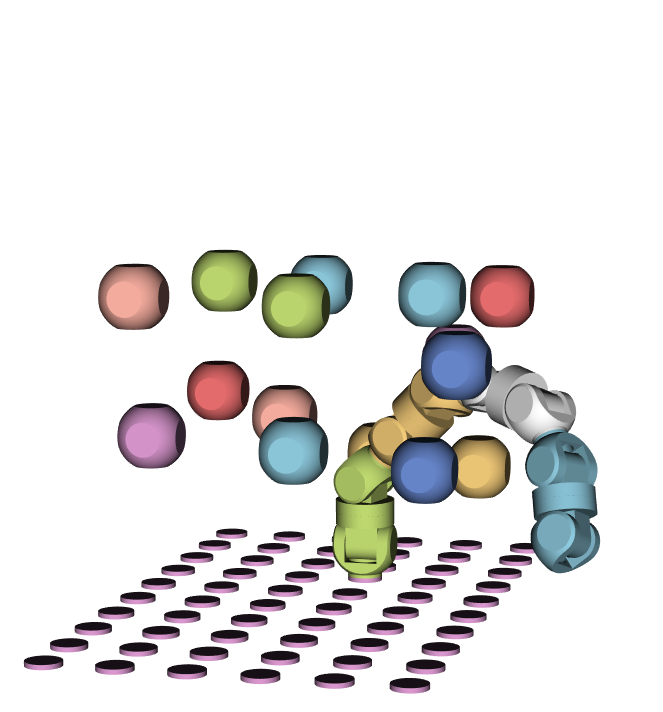
\includegraphics[width=0.245\textwidth]{sim7_3.png}

    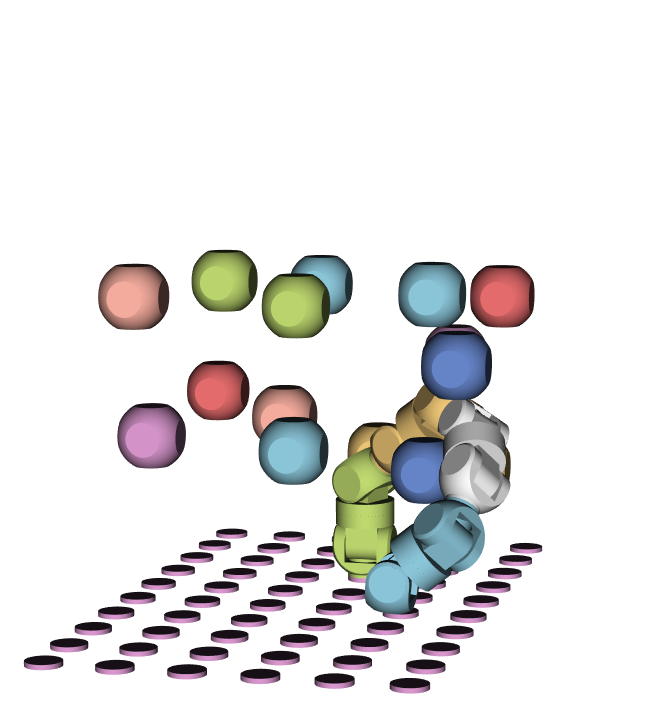
\includegraphics[width=0.245\textwidth]{sim7_4.png}
    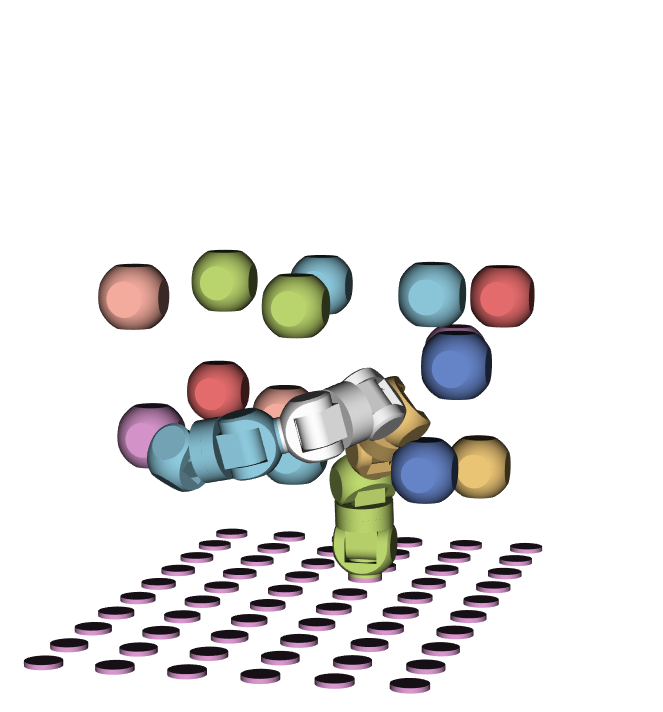
\includegraphics[width=0.245\textwidth]{sim7_5.png}
    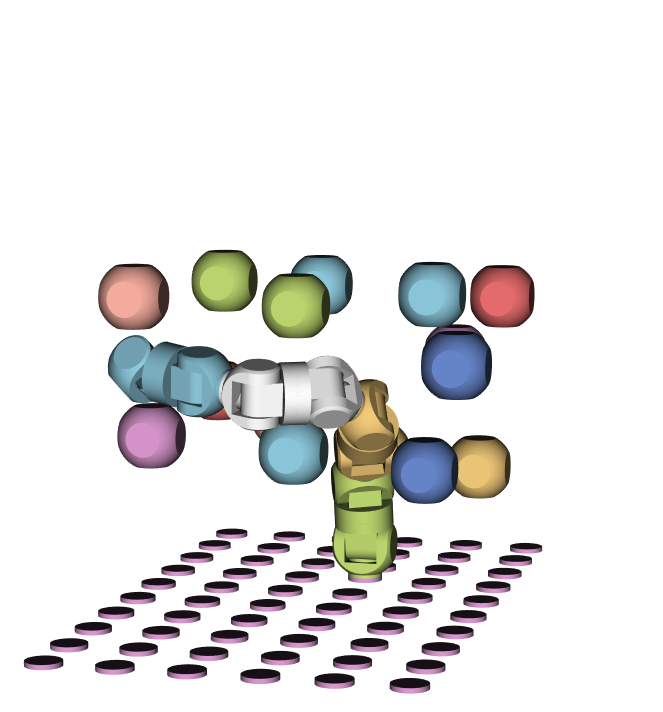
\includegraphics[width=0.245\textwidth]{sim7_6.png}
    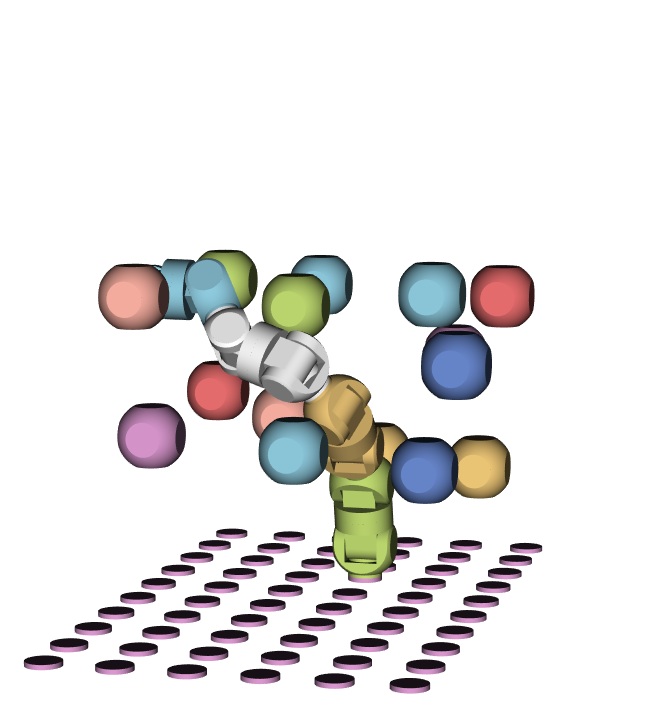
\includegraphics[width=0.245\textwidth]{sim7_7.png}
  \end{minipage}
  \caption{Obstacles all around}\label{fig:sim7}
\end{figure}

The average number of explored paths is higher in this case, and the found paths can stray further from the optimal one. In some cases, the algorithm finds a path close to the expected solution, but since the obstacles in the way have no effect on the resulting path, the manipulator does not always find suitable intermediate positions on this path. Even so, the algorithm is capable of navigating through very complex environments, see Figure~\ref{fig:sim7}. We can see that the path of the \textit{end effector} is quite long, and was obviously not the first found solution; it was the 13\th{} path, found after $2$ seconds.

As we can see, the algorithm performs nicely in various environments and finds successful ways to reach the given target. The computation usually runs for less than a second, instantaneous in eyes of a human observer. Reaching some targets takes a couple of seconds, leading to a noticeable delay, but note that the implementation is only a proof of concept, and the given times are referential; there are certainly more optimisations that can be added to the algorithm.

Target examples are included as a video in the thesis archive with the complete motion:

\begin{itemize}
\item \textsc{around\_wall.mp4} shows an example of reaching back to avoid a wall
\item \textsc{through\_hole.mp4} shows getting through a small hole
\item \textsc{obstacles\_near\_target.mp4} shows reaching for a target in the middle of other obstacles
\item \textsc{obstacles\_around.mp4} shows the manipulator navigating through a complex environment with obstacles all around
\end{itemize}

\newpage

\section{Dissecting the algorithm}

To delve deeper into analyzing our algorithm, we can look at some of the previous examples and evaluate which parts are the most expensive. We measure the following parameters:

\begin{itemize}
\item Initialization, which includes building an AABB with all the obstacles and creating the graph
\item Djikstra, which looks for shortest paths in the created graph
\item FABRIK, which serves to find manipulator positions on the found paths
\item Interpolation between the positions computed by FABRIK, to see if a step is valid and whether it can be skipped
\end{itemize}

\begin{figure}[ht]
  \centering
  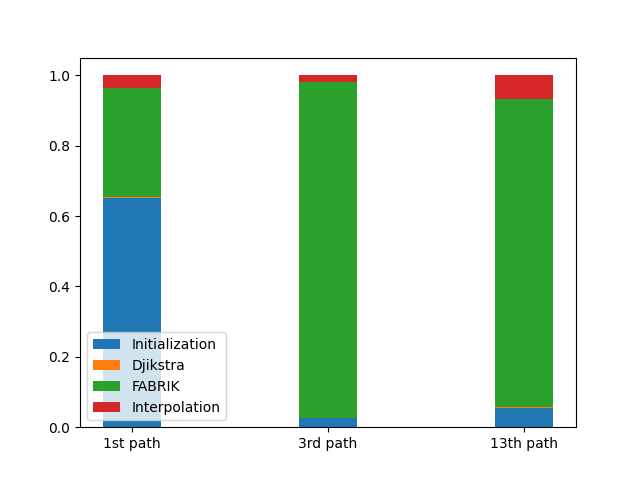
\includegraphics[width=0.5\textwidth]{Runtimes.png}
  \caption{Percentage of computation times for each component}\label{fig:percentage}
\end{figure}

Figure~\ref{fig:percentage} shows 3 examples: The first one is an environment with 12 obstacles, but the target is trivially reachable. The second example is a nontrivial target in the same environment, and the third is a target far from the manipulator in a space with 20 randomly generated obstacles. The total runtimes are $0.01s, 0.7s, 2.3s$ respectively. In the first bar, the initialization is seemingly expensive compared to the other parts of the computation. However, looking at the 2\nd{} and 3\rd{} examples, it becomes obvious that the repeated FABRIK computation is the heavy part: although a single computation is very fast, particularly when making incremental changes, we have to compute it many times. In addition, reaching a target is significantly faster than determining that a target is not reachable, which adds a lot of extra cost to unsuccessful paths. As direction for where the algorithm can be optimised, we can look at ways of shutting down computations for unsuccessful paths early and reducing the number of unsuccessful FABRIK computations.

On the other hand, since our representation of space is compact, finding shortest paths with Djikstra takes barely any time, hence, trying to optimize this part with something like A* would bring no benefit. Since this part is so cheap, a possible improvement could be adding more control points throughout the manipulator's workspace and finding successful ways to reach the target sooner.

\begin{wrapfigure}{l}{0.4\textwidth}
  \centering
  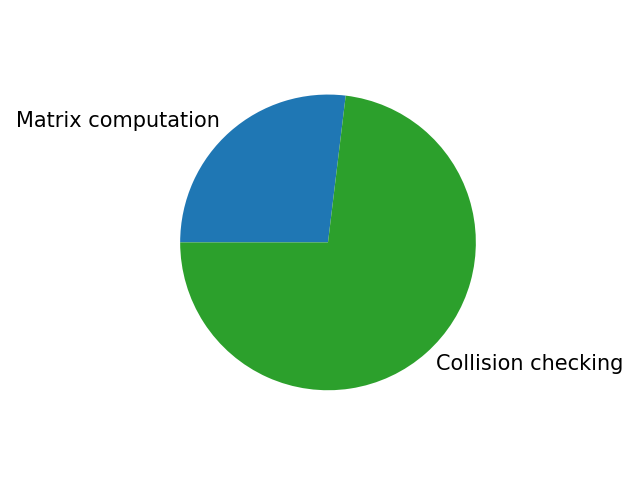
\includegraphics[width=0.4\textwidth]{fabrik_anal.png}
  \caption{\\Computation times within FABRIK}
\end{wrapfigure}

Since we've extended FABRIK to compute with matrices instead of points and check for collisions, it is worth analyzing which parts of FABRIK make it slow down. The piechart shows the rate of the respective computation times when running in an environment with 20 obstacles. Collision checking includes all the work associated with the AABB tree management, while the remaining time deals with finding the right joint angles and computing the respective transformation matrices. As we can see, the extension to various joints with limits does not slow the algorithm down in a significant way, but avoiding collisions with nearby objects does.

\section{Exploring the Limits}

In Section~\ref{study}, we have shown how the algorithm deals with various handcrafted examples. In most cases, a solution was found quickly, and a smooth motion was performed. However, since the whole approach is heuristic, we need to analyse how it performs in various situations. We can parametrize various types of obstacles via their defining aspects and evaluate them individually.

There are a few main aspects we can parametrize the algorithm with respect to: the number of joints, the number of obstacles, the shapes that the obstacles form, and the distance between the individual obstacles.

First up, we can confirm that the algorithm scales well with respect to the joints only. For this purpose, we can test it out in an environment with very few obstacles, and generate random targets unobstructed by any of the obstacles. Figure~\ref{fig:scaling} shows the average computation time among reaching 10 consequent targets. Since the expensive part of the algorithm lies in FABRIK, we get a nice linear looking scaling. This scaling is a critical aspect of the algorithm: since each module brings 3 extra degrees of freedom, not only does the algorithm work for 12 DoF, double the state of the art amount, it scales reasonably well into 30.

\begin{figure}
  \centering
  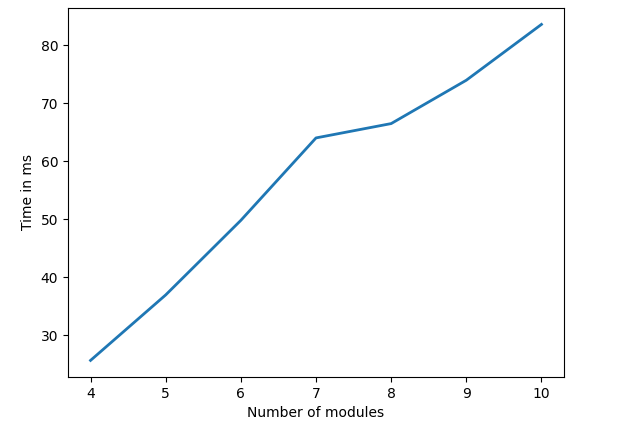
\includegraphics[width=0.5\textwidth]{scaling.png}
  \caption{Increase in computation time with longer manipulators}\label{fig:scaling}
\end{figure}

Although we've estimated the asymptotical complexity of the extended FABRIK higher than linear, the AABB operations are not significantly more expensive with the addition of a few joints.
The paths, which can be quite a bit longer due to the manipulator's extended reach, can make a big difference in how many times FABRIK is computed. The difference does not show itself in this particular case because we know we can choose the shortest one, as well as make large intermediate steps when there are no obstacles on the chosen path.

Next up, we can analyze the behaviour of the algorithm around obstacles that form walls. As reference for measuring distance, we will use the diameter of a single joint as $1$ unit of distance; then, a single universal module is $1$ unit wide and $2$ units high. Naturally, in order for the manipulator to fit between two of our obstacles, the distance between them has to be greater than $1$.

Getting around a single wall, as in Figure~\ref{fig:sim4}, poses no problem regardless of where the target lies, as long as it is within the manipulator's reach. Since the required motion to go around any single wall is relatively straightforward, the algorithm finds ways to go around, behind, as well as over any wall with ease.

Getting between a pair of walls is similarly straightforward. We have already shown that our algorithm is capable of dealing with a small hole in a wall; the problem of getting between 2 walls is a simplified version. The algorithm only needs a bit of space to move around; as long as the walls are spaced out at least $1.1$ units apart, we find solutions quickly and reliably (see Figure~\ref{fig:2walls}).

\begin{figure}
  \centering
  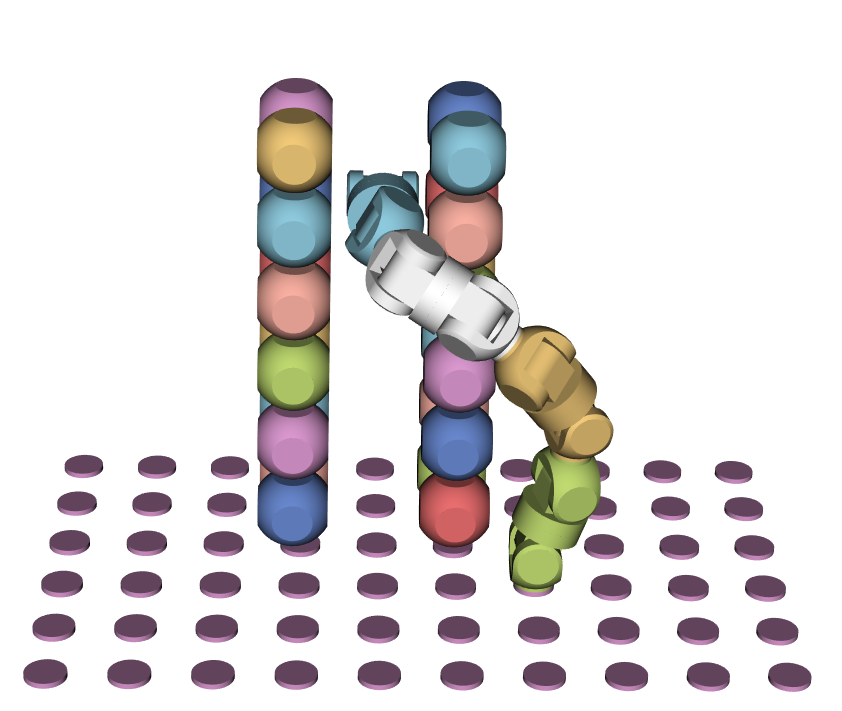
\includegraphics[width=0.5\textwidth]{between_walls.png}
  \caption{Reaching a target between two walls}\label{fig:2walls}
\end{figure}


Walls start to pose a problem when they form corridors that the manipulator needs to navigate through. Since the algorithm is designed to avoid narrow passageways between obstacles if at all possible, the paths that may seem natural from a human standpoint, which result in the manipulator crawling between the obstacles, are evaluated as too expensive. In order to achieve motion that passes through the corridor, as in Figure~\ref{fig:corridor}, we need to specify intermediate targets on the path explicitly. By default, the algorithm unsuccessfully looks for ways to avoid the passageway altogether.

\begin{figure}[ht]
  \centering
  \begin{minipage}{0.9\textwidth}
    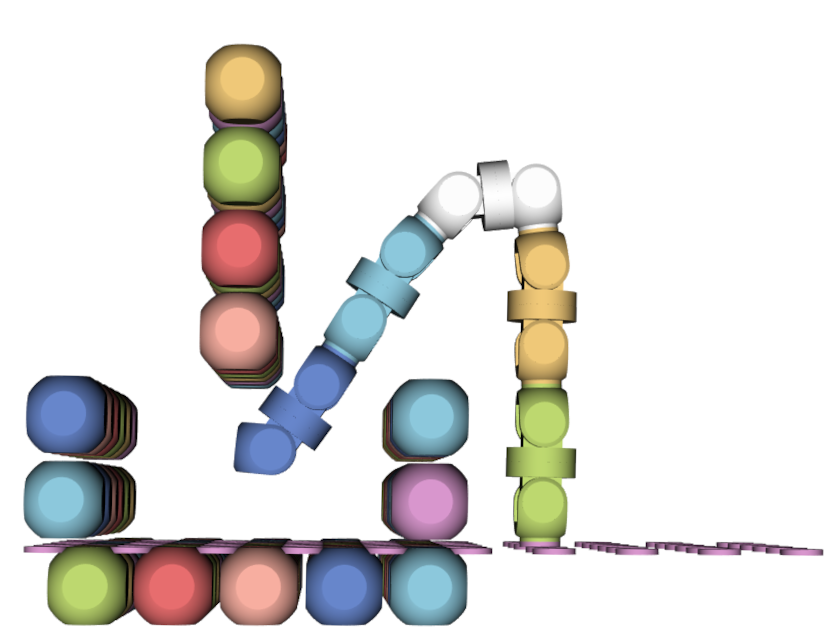
\includegraphics[width=0.5\textwidth]{corridor1.png}
    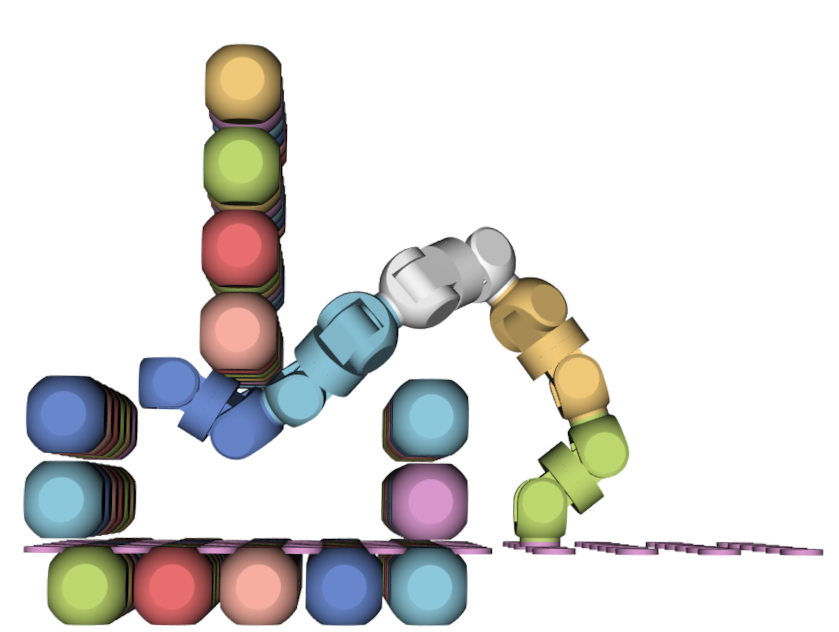
\includegraphics[width=0.5\textwidth]{corridor2.png}
  \end{minipage}
  \caption{Navigating through a corridor}\label{fig:corridor}
\end{figure}

We can parametrize corridors with respect to the number of walls that the manipulator needs to crawl around, as well as the distance between the walls. If there are at least $3$ walls spaced out at less than $3$ units apart, the algorithm does not find viable solutions even though they exist. This makes the procedure completely unsuitable for this particular scenario. In order to adapt the algorithm to deal with corridors and narrow passageways, we would have to tweak the graph generation and not assign higher weights to the points that lead through obstacles; or extend the algorithm with a way to find intermediate targets in the corridor.

We've shown that the algorithm can pass through narrow holes (Figure~\ref{fig:sim5}), but claimed that it can struggle with particular cases. The notion can be quantified via the size of the hole. If the hole is at least $1.5$ units wide, the algorithm finds solutions without any problems. If the hole is narrower, and the target lies beyond the hole, reaching for the target is no longer as reliable.

In order to fully evaluate whether this is a suitable margin, we would need to specify the expected use case for the algorithm. As a general algorithm, we can consider it acceptable. For instance, if we are using the manipulator to pick and place objects out of a box, it is fully sufficient.
However, much like in the previous case, if we expect to encounter narrow passageways a lot, we need to extend the algorithm to generate intermediate targets, or assign lower costs to these passageways to find paths through them more reliably.

There is not much to say about the algorithm dealing with clusters near the target. Due to the way the algorithm is designed, the manipulator consistently reaches its target without any issues.

Finally, we can take our original manipulator of 4 modules and test it out with an increasing number of randomly placed obstacles. For reference, see Figure~\ref{fig:sim7}: obstacle positions are generated in a way that they do not form clusters, but instead occupy different parts of the manipulator's workspace. Each additional obstacle is generated so that it is at least $0.5$ units from every other obstacle. This way, we can evaluate the algorithm at a larger scale, as we take away an increasing amount of space away from it. With this setup, we can simply parametrize the environemnts with respect to the number of obstacles.

We generate 100 random subsequent targets for the manipulator, and see how many were reached and how long it took to find a viable path. Since determining whether a point is reachable in itself is a hard problem, we settle with generating targets in the manipulator's range that do not collide with any obstacles. The goal may not be reachable due to the rotation of the end effector or a particular way obstacles were generated, which can lead to a false negative. Even so, it gives us a lower bound on the success rate of our algorithm.

\begin{figure}
  \centering
  \begin{subfigure}{.45\textwidth}
    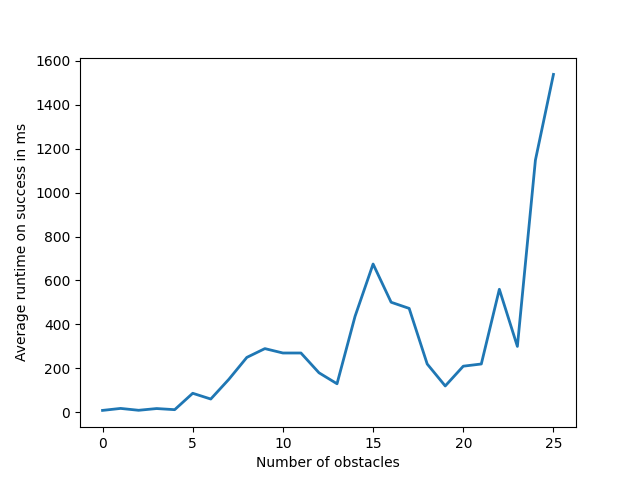
\includegraphics[width=0.99\textwidth]{obstacle_times.png}
    \caption{Number of obstacles and the average time to reach a target}
  \end{subfigure}
  \begin{subfigure}{0.45\textwidth}
    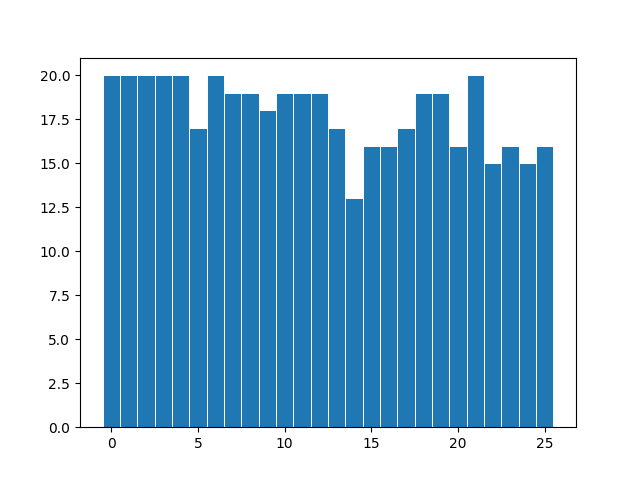
\includegraphics[width=0.99\textwidth]{obsacle_success.png}
    \caption{Number of obstacles and the success rate}
  \end{subfigure}

  \caption{Manipulator of 4 modules with random targets between randomly generated obstacles}\label{fig:inc_obst}
\end{figure}

As we can see in Figure~\ref{fig:inc_obst}, the manipulator can move around very well all the way up to 25 obstacles, finding solutions with a high success rate in up to a second of time. Unfortunately, 25 obstacles seems to be the limit for RoFI manipulators of 4 modules, as a higher count no longer gave the manipulator around space to move around and trying to reach most targets failed.

\begin{figure}
  \centering
  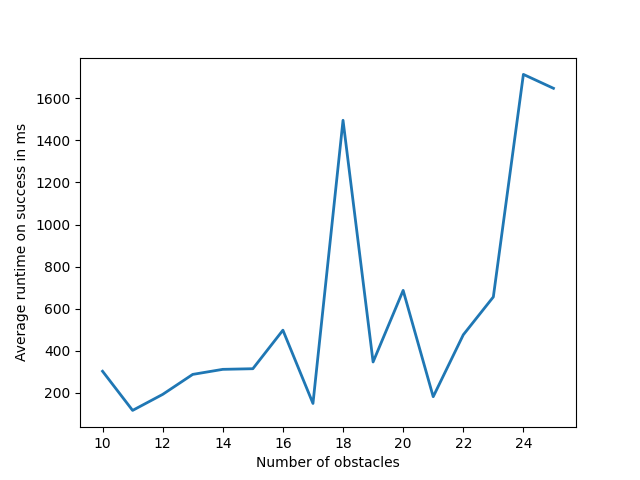
\includegraphics[width=0.4\textwidth]{obstacle_times5.png}
  \caption{Number of obstacles and the average time to reach a target for 15-DoF manipulator}\label{fig:5modules}
\end{figure}

To test out the scalability of our algorithm, we can take our randomly generated environments and see how the algorithm performs with a higher number of joints as well as obstacles. When we take randomly generated environments and add a few additional modules, we can observe that the average time to reach a target is higher, but still comparable. Figure~\ref{fig:5modules} shows the average time to reach a target when we add an extra module to our original manipulator. Even though the cost of individual operations is higher, the average number of explored paths is lower due to the higher flexibility of the robot.

Clearly, we have achieved our main goal: the algorithm scales very well with respect to an increasing number of joints as well as obstacles. With 15 degrees of freedom, we have successfully more than doubled the number of DoF the algorithm is suitable for, compared to the state of the art.

With that, we can conclude the evaluation of our algorithm. We have shown that it generates naturally looking trajectories, the computation is fast, and has a high success rate. The algorithm excels at dealing with obstacles near the target position, and it can navigate through environments with random obstacles throughout the space, as well as get around walls. One particular weakpoint of the approach is trying to get through narrow corridors: for this purpose, the algorithm would need to be tweaked further.
